\chapter{Evaluation}

This chapter presents an evaluation of the constraints when applied to a number of open source systems. The evaluation was performed in two ways: first a comparison between SecArchUnit and static analysis tools used in industry, and then a standalone evaluation of the tool extension.

\section{Comparison with Industry Tools}
As mentioned in Section~\ref{sec_tools_used_in_comparison}, constraints 1-5 can be validated in both SonarQube and PMD through the definitions of custom rules. The constraints are applied to the test systems presented in Section~\ref{sct:selected-systems} and validated using each of the three tools. Both the relative and absolute frequencies of violations of each constraint can be seen in Figure~\ref{bar:rel_frequency_violation_compraison} and Figure~\ref{bar:frequency_violation_compraison} respectively.

\begin{figure}[h]
  \centering
  \captionsetup{justification=centering}
  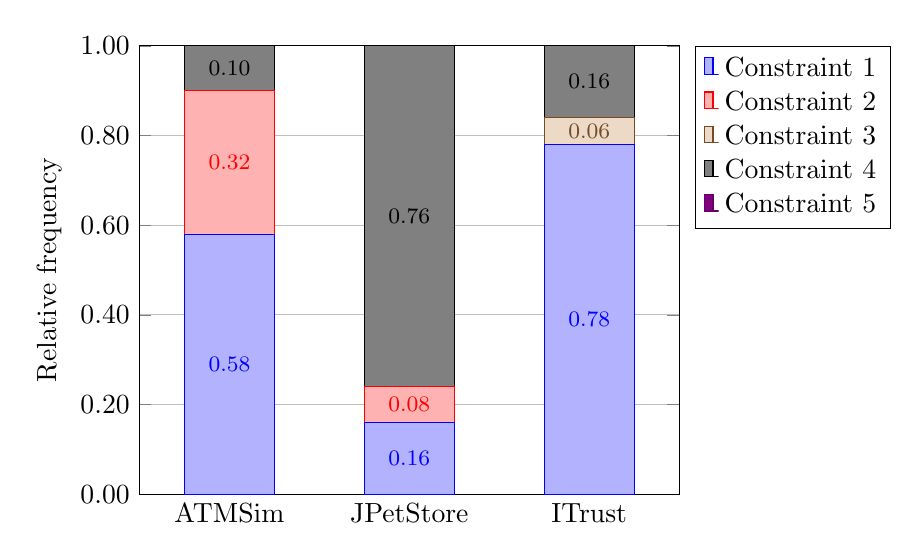
\begin{tikzpicture}\pgfkeys{
     /pgf/number format/precision=2, 
    /pgf/number format/fixed zerofill=true,
    /pgf/number format/fixed
}
  
    \begin{axis}[
        ybar stacked,
        ymajorgrids = true,
        nodes near coords,
        every node near coord/.append style={font=\footnotesize},
        xbar legend,
%         nodes near coords align={right},
        legend pos=outer north east,
        enlarge x limits=0.25,
        enlarge y limits=false,
        bar width=.5,
        % x axis
        xtick={1,2,3},
        xticklabels={ATMSim,JPetStore,ITrust},
        %x tick label style={rotate=45,anchor=east},
        % y axis
        ymin=0,
        ylabel={Relative frequency},
      ]
     % C1
     \addplot+[ybar] plot coordinates {(1,0.58) (2,0.16) 
      (3,0.78)};
     % C2
    \addplot+[ybar] plot coordinates {(1,0.32) (2,0.08) 
      (3,0)};
     % C3
    \addplot+[ybar] plot coordinates {(1,0) (2,0)
      (3,0.06)};
     % C4
    \addplot+[ybar] plot coordinates {(1,0.1) (2,0.76) 
      (3,0.16)};
     % C5
    \addplot+[ybar] plot coordinates {(1,0) (2,0) 
      (3,0)};
      

      \legend{Constraint 1,Constraint 2,Constraint 3, Constraint 4, Constraint 5}
    \end{axis}
  \end{tikzpicture}

  \caption{The relative frequency of constraint violations found in the three projects.}
  \label{bar:rel_frequency_violation_comparison}
\end{figure}
\begin{figure}
\centering
\captionsetup{justification=centering}

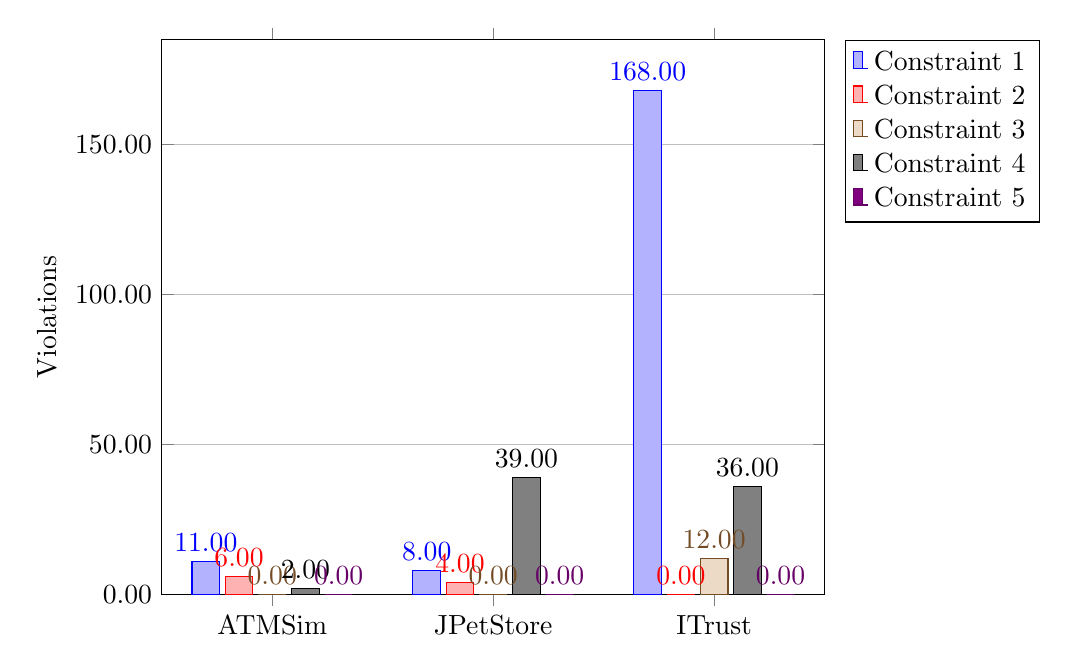
\begin{tikzpicture}
\begin{axis}[
    width=10cm,
    ybar,
    ymin = 0,
    ymajorgrids = true,
    enlarge x limits=0.25,
    xbar legend,
    legend pos=outer north east,
    ylabel={Violations},
    symbolic x coords={ATMSim,JPetStore,ITrust},
    %xlabel={System},
    xtick=data,
    nodes near coords,
    nodes near coords align={vertical},
    ]
%C1
\addplot coordinates {(ATMSim,11) (JPetStore,8) (ITrust,168)};
%C2
\addplot coordinates {(ATMSim,6) (JPetStore,4) (ITrust,0)};
%C3
\addplot coordinates {(ATMSim,0) (JPetStore,0) (ITrust,12)};
%C3
\addplot coordinates {(ATMSim,2) (JPetStore,39) (ITrust,36)};
%C3
\addplot coordinates {(ATMSim,0) (JPetStore,0) (ITrust,0)};
\legend{Constraint 1,Constraint 2,Constraint 3, Constraint 4, Constraint 5}
\end{axis}
\end{tikzpicture}

\caption{The constraint violations found in the ground truth of each system.}
\label{bar:frequency_violation_comparison}
\end{figure}

As shown in the figures, the tools were evaluated using imbalanced data. Constraint 1 accounted for a majority of all violations found throughout all three systems, while no system violated constraint 5. Addtionally, iTrust was the only system to contain a violation of constraint 3. 

Each tool is evaluated according to the performance metrics, i.e. precision and recall. These results are presented in Table~\ref{tab:results_comparison}. Both in regards to precision, as well as recall, the tools performed equally. However, the causes of failure, in cases where the results of the tools varied, differed noticeably. The examples are described below:

\begin{itemize}
    \item In ATM simulator, the same false positive occurred in all three tools. This was in relation to constraint 3, where a subclass of the sending point contained a method call to the sender. Additionally, PMD had 4 false negatives which occurred because it was unable to determine the classes that these method calls targeted.
    \item In JPetStore, PMD reported 4 false negatives, again because it was unable to determine the target class of these method calls.
    \item In iTrust, a security service contained both an inner interface and an inner static class whose methods did not perform any security events. In both PMD and SonarQube, these methods were determined to be declared in the inner class by traversing the AST from the method to its first parent class or interface declaration. In comparison, ArchUnit considers the members of the inner class to be declared in both the inner and outer class. This improperly marks the inner methods as violating the constraint, resulting in 3 false positives.
\end{itemize}

\newcolumntype{g}{>{\columncolor{RowColor}}c}
\newcolumntype{x}{>{\columncolor{RowColor}}l}
\begin{table}[h]
\begin{center}
\begin{tabular}{lxggggg}
\rowcolor{white}
\textbf{Project}           & \textbf{Tool}    & \textbf{TP} & \textbf{FP} & \textbf{FN} & \textbf{Precision} & \textbf{Recall} \\
\hline
\rowcolor{white}
\multirow[t]{3}{*}{ATMsim}    & SecArchUnit      & 19          & 1           & 0           & 1               & 0.95            \\
                           & SonarQube Plugin & 19          & 1           & 0           & 1               & 0.95            \\
                           \rowcolor{white}
                           & PMD Plugin       & 15          & 1           & 4           & 0.94               & 0.79            \\
\hline
\rowcolor{white}
\multirow[t]{3}{*}{JPetStore} & SecArchUnit      & 51          & 0           & 0           & 1                  & 1               \\
                           & SonarQube Plugin & 51          & 0           & 0           & 1                  & 1               \\
                           \rowcolor{white}
                           & PMD Plugin       & 47          & 0           & 4           & 1                  & 0.92            \\
\hline
\rowcolor{white}
\multirow[t]{3}{*}{ITrust}    & SecArchUnit      & 216         & 3           & 0           & 0.97               & 1               \\
                           & SonarQube Plugin & 216         & 0           & 0           & 1                  & 1               \\
                           \rowcolor{white}
                           & PMD Plugin       & 216         & 0           & 0           & 1                  & 1 \\
\hline
\end{tabular}
\end{center}
\caption{Results from validating constraints 1-5 using SecArchUnit, SonarQube and PMD.}
\label{tab:results_comparison}
\end{table}

\section{Validation of ArchUnit Extension}
Constraints 6-7, which rely on an extension of ArchUnit's analysis, are validated solely using SecArchUnit. The performance metrics from applying the final two constraints to iTrust are presented in Table~\ref{tab:tool_extension}.

The system, iTrust, initially contained no violations of constraint 7. Therefore, violations were injected by systematically marking all identifier fields (e.g. \texttt{patientId}, \texttt{personnelId}) in the model and base-action packages as secrets. We chose to mark these identifiers because they were commonly sent to the logger as a way to describe the patient or personnel involved in a transaction. Hence, the 37 violations of constraint 7, as seen in Table~\ref{tab:tool_extension}, are artificially injected.

Moreover, iTrust is built with a mix of Java and Java Server Pages (JSP) files whereas ArchUnit can only analyze plain Java. The classes in the action package, from which the logger is called, are all instantiated in the JSP files outside the view of our analysis. As such, the types of information flow that are analyzed and included in the ground truth are rather rudimentary. Out of the 37 violations of constraint 7, 1 was found without recursion (direct access to secret field) and the remaining 36 were found using a single recursion step (access to getter method of a secret field).
% This is bad - we could just as well put the secret annotation on the getter and enforce the same constraint in SonarQube/PMD

\begin{table}
\begin{center}
\begin{tabular}{lccccc}
\hline
\textbf{Constraint} & \textbf{TP} & \textbf{FP} & \textbf{FN} & \textbf{Precision} & \textbf{Recall} \\
\hline
6 & 24 & 0 & 0 & 1 & 1\\
\rowcolor{RowColor}
7 & 37 & 0 & 0 & 1 & 1\\
\hline
\end{tabular}
\end{center}
\caption{Results from validating the extension-based constraints on iTrust.}
\label{tab:tool_extension}
\end{table}